\chapter{Elektromotoren steuern}\label{kap:elektromotoren}
\label{kap:e-motor}
% kurz: Aufbau eines Motors
% mögliche rückläufige Induktionsströme durch Diode aufhalten
% Erklärung Diode als Ventil; Umwandlung von Energie in Wärme statt Licht
% Achtung: Falls Diode falsch angebracht, dann kann Arduino oder Transistor zerstört werden!
% Schaltplan ohne transistor (an 5V und GND, MIT Diode)
% Schaltplan mit Transistor (macht Schalterfunktion deutlich)
% Schaltplan mit externer Spannungsquelle; gemeinsamer GND
% Ansteuerung mit analogWrite
Erst mit Motoren werden elektrischen Schaltungen dazu befähigt, mechanisch in ihre Umgebung einzugreifen, \emph{etwas zu tun}. Die bereits kennengelernten Servos haben dies auch schon ermöglicht, dienen aber eher für Steuerungen, die eine Feinjustierung benötigen. Größere Aufgaben bewältigt der Elektromotor.

\bigskip
In diesem Kapitel lernst du\dots
\begin{itemize}
	\item \dots wie man einen Elektromotor richtig am Arduino anschließt,
	\item \dots wie man einen Elektromotor mit einem Transistor steuert,
	\item \dots wie man einen Elektromotor mit einem Relais steuert,
	\item \dots wie man einen Elektromotor mit einem Motortreiber-IC steuert,
	\item \dots welche Vorteile und Nachteile die jeweiligen Steuerungsarten bieten.
\end{itemize}

\bigskip

\begin{projektueberblick}
	\item Badezimmerlüfter \dotfill \pageref{proj:badezimmerluefter}
	\item Waschmaschinensteuerung \dotfill \pageref{proj:waschmaschinensteuerung}
\end{projektueberblick}

\newpage
\section{Elektromotor und Diode}

\marginpar{%
	\footnotesize%
	\zurueck 
	\hyperref[sec:transistor]{Mit Transistoren steuern}
}
Bei vielen Projekten soll sich etwas bewegen - dies lässt sich mit Elektromotoren realisieren. Die Ansteuerung eines Elektromotors erfordert auf der Hardware-Seite ein wenig Vorbereitung, denn aufgrund der hohen Ströme, die Elektromotoren ziehen, sollte man sie nicht direkt an den Digitalpins des Arduino anschließen. Für die Steuerung greift man meistens auf einen Transistor zurück; eine brauchbare Alternative ist aber auch das Relais. Für beide Steuerungsmöglichkeiten sollte aber zuerst geklärt werden, wie ein Motor grundsätzlich aufgebaut und betrieben wird.

\begin{ziel}
	\textbf{Frage:} Wie betreibt man einen Elektromotor am Arduino?
\end{ziel}

\begin{wrapfigure}{r}{0.38\textwidth}
	\centering
	\hfill
	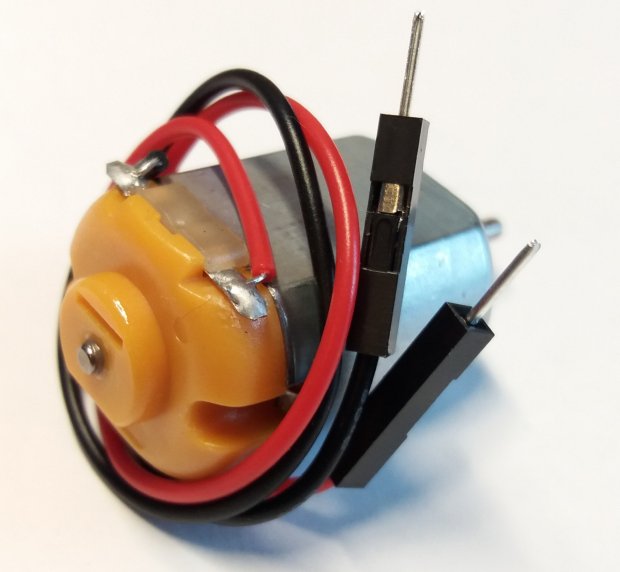
\includegraphics[width=0.21\textwidth]{./pics/dc-motor-klein.png}
	\hfill
	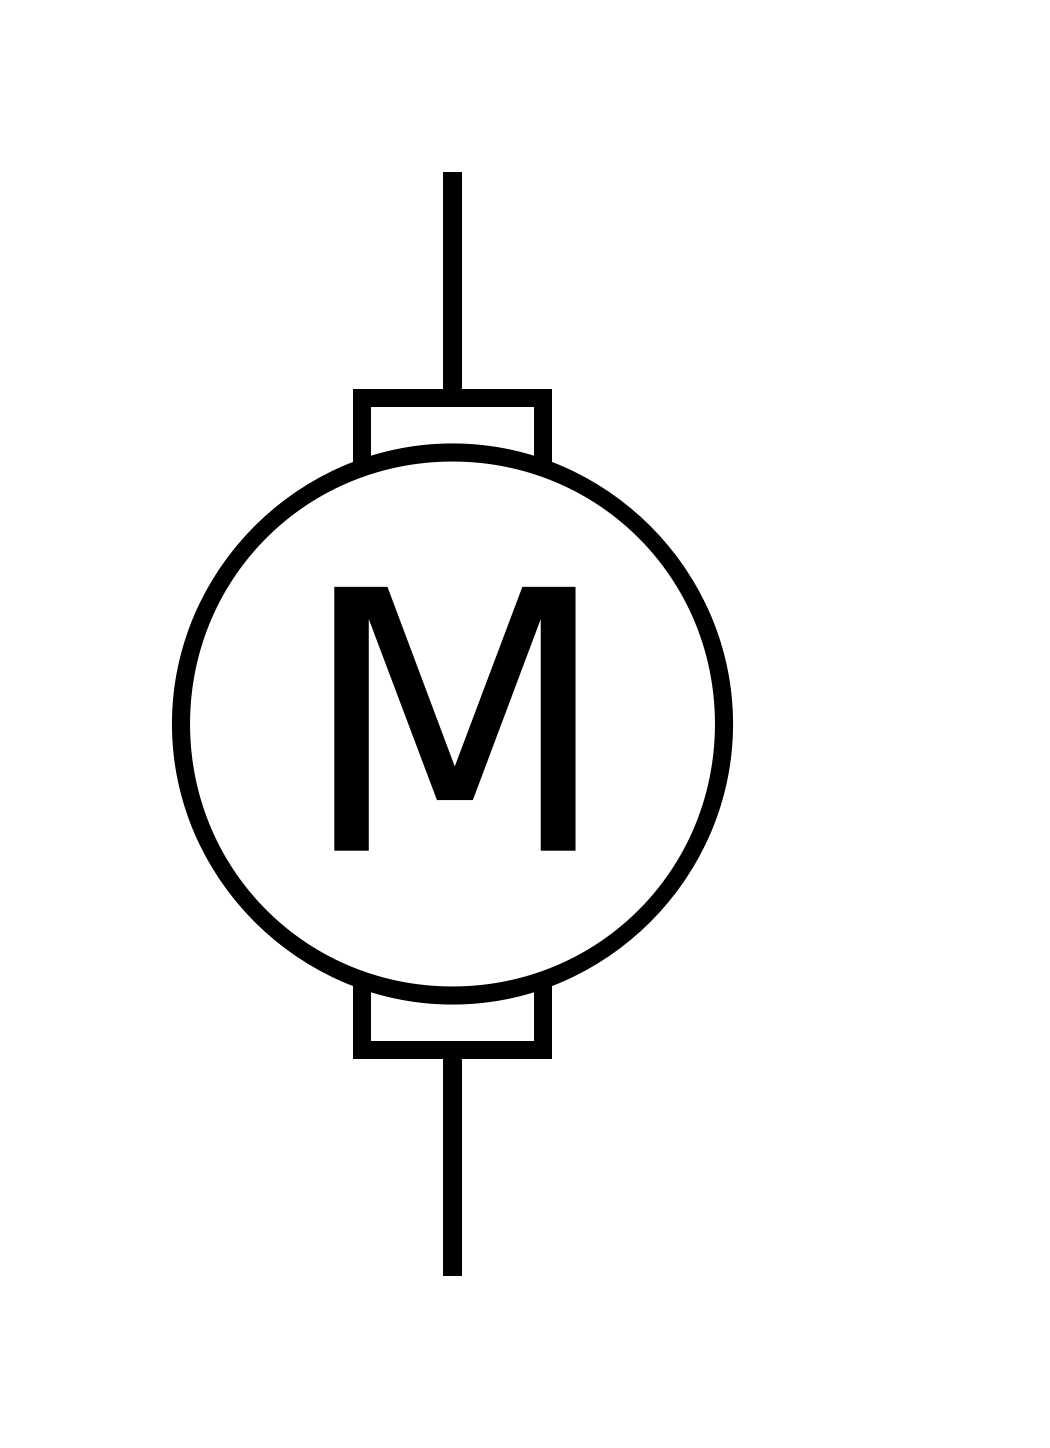
\includegraphics[width=0.13\textwidth]{./Zeichnungen/motor-schaltsym.png}
	\hfill
	\caption{Gleichstrom-Elektromotor in real und als Schaltsymbol.}
\end{wrapfigure}
Ein \textbf{Elektromotor} besteht aus mehreren Spulen und Magneten. Wenn Strom durch die Spulen fließt, baut sich um die Spulen ein Magnetfeld auf, das mit dem Magnetfeld der eingebauten Magneten wechselwirkt (Anziehung/Abstoßung), sodass es zu einer Drehung des Motors kommt. Ein sogenannter Kommutator sorgt dafür, dass der Strom durch die Spulen ständig seine Richtung wechselt, sodass es immer wieder von Neuem zu Anziehung bzw. Abstoßung der Magnetfelder kommt und die Drehung nicht aufhört, solange eine Spannung anliegt.

%\medskip
%\begin{minipage}{0.6\textwidth}
%	Ein Elektromotor besteht aus mehreren Spulen und Magneten. Wenn Strom durch die Spulen fließt, baut sich um die Spulen ein Magnetfeld auf, das mit dem Magnetfeld der eingebauten Magneten wechselwirkt (Anziehung/Abstoßung), sodass es zu einer Drehung des Motors kommt. Ein sogenannter Kommutator sorgt dafür, dass der Strom durch die Spulen ständig seine Richtung wechselt, sodass es immer wieder von Neuem zu Anziehung bzw. Abstoßung der Magnetfelder kommt und die Drehung nicht aufhört, solange eine Spannung anliegt.
%\end{minipage}
%\hfill
%\begin{minipage}{0.38\textwidth}
%	\centering
%	\hfill
%	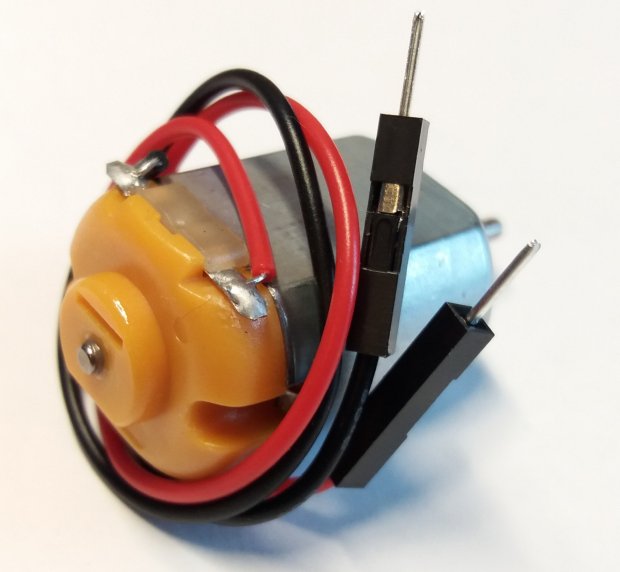
\includegraphics[width=0.55\textwidth]{./pics/dc-motor-klein.png}
%	\hfill
%	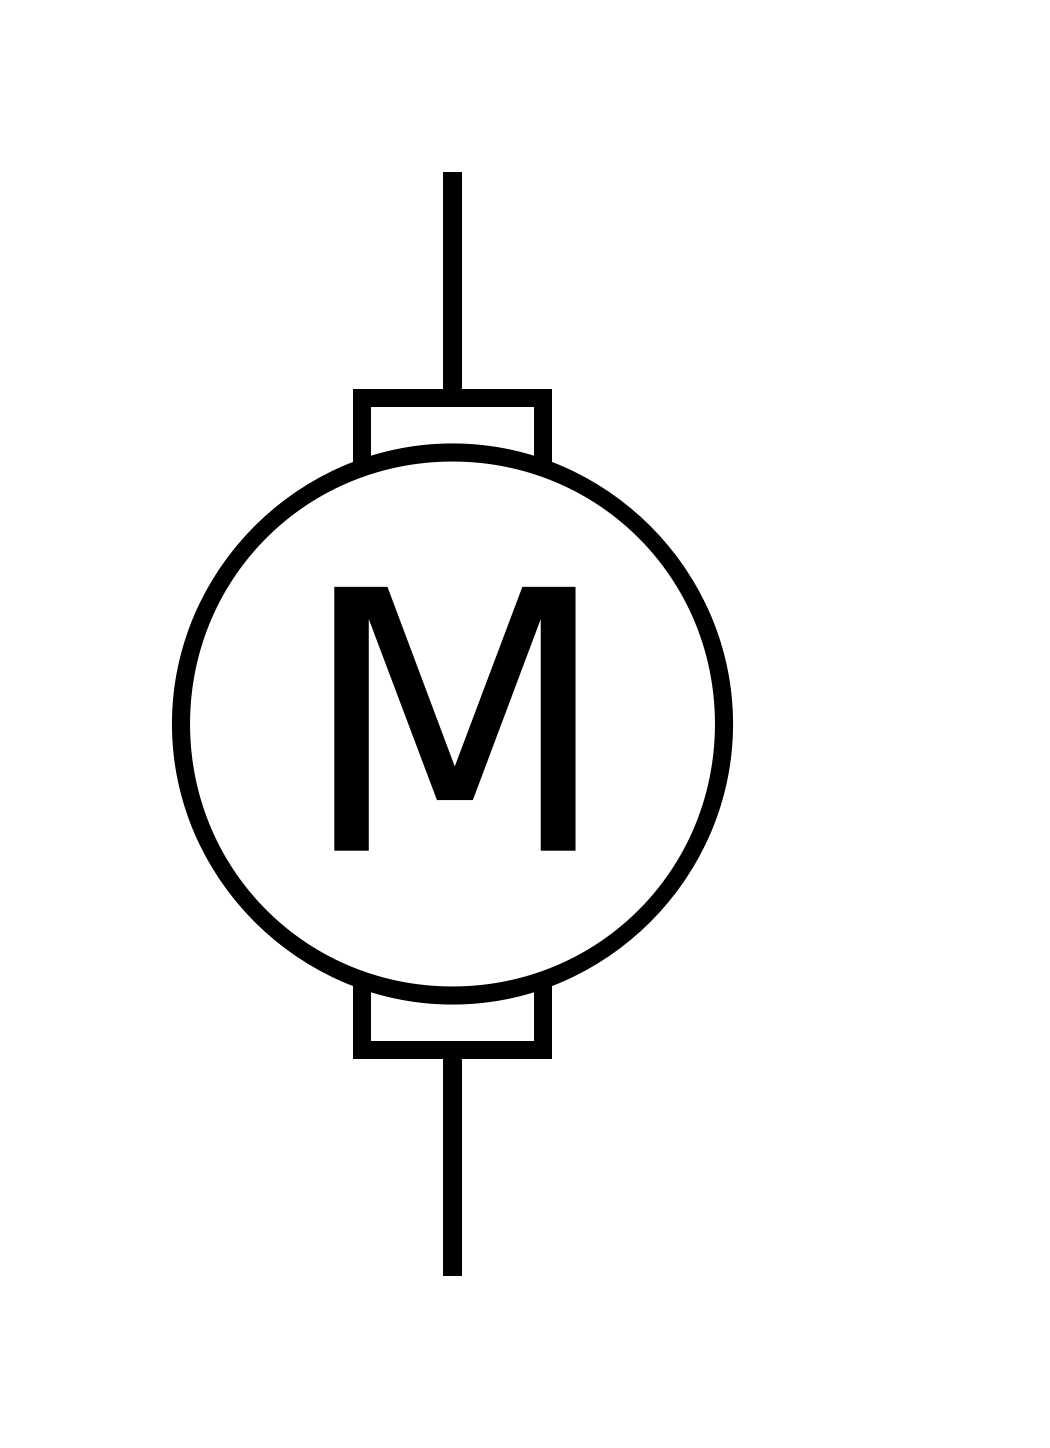
\includegraphics[width=0.35\linewidth]{./Zeichnungen/motor-schaltsym.png}
%	\hfill
%\end{minipage}
%\medskip

Wenn keine Spannung mehr am Motor anliegt, wird sich der Motor aufgrund seiner Trägheit immer noch ein wenig weiterdrehen. Durch das Drehen der Spulen im Magnetfeld der eingebauten Permanentmagneten wird in den Spulen ein Strom induziert, dessen Richtung entgegengesetzt zur vorherigen Richtung ist. Dieser \enquote{falsch} gerichtete Strom würde den Arduino zerstören. Aus diesem Grund schaltet man eine \emph{Diode} parallel zum Motor.

\begin{wrapfigure}{r}{0.28\textwidth}
	\centering
	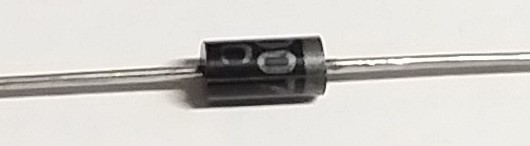
\includegraphics[width=0.75\linewidth]{./pics/diode2.jpg}
	
	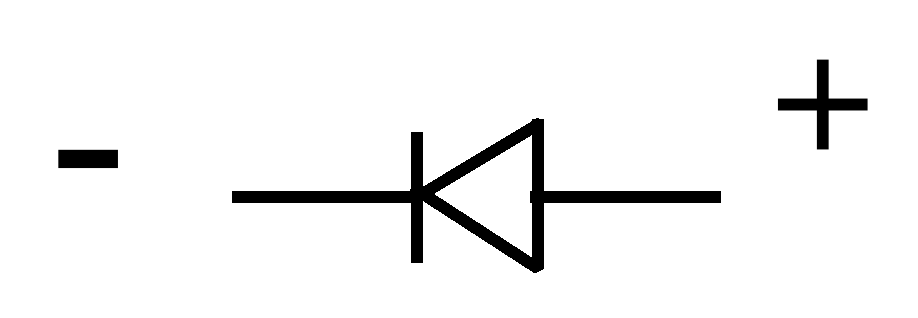
\includegraphics[width=0.75\linewidth,angle=180]{./Zeichnungen/diode-schaltsym.png}
	\caption{Diode in real und als Schaltsymbol.}
\end{wrapfigure}
Eine \textbf{Diode} ist wie ein elektrisches Ventil: Sie lässt den Strom nur in eine Richtung durch. Im Gegensatz zu Leuchtdioden wandeln \enquote{normale} Dioden die elektrische Energie in Wärme um. In \emph{Durchlassrichtung} wird der negative Pol (bzw. GND) mit der Seite verbunden, an der der Ring angebracht ist, und der positive Pol mit der anderen Seite.

%\medskip
%\begin{minipage}{0.7\textwidth}
%	 Eine Diode ist wie ein elektrisches Ventil: Sie lässt den Strom nur in einer Richtung durch. Im Gegensatz zu Leuchtdioden wandeln \enquote{normale} Dioden die elektrische Energie in Wärme um. In Durchlassrichtung wird der negative Pol (bzw. GND) mit der Seite verbunden, an der der Ring angebracht ist, und der positive Pol mit der anderen Seite.
%\end{minipage}
%\hfill
%\begin{minipage}{0.28\textwidth}
%	\begin{figure}[H]
%		\centering
%		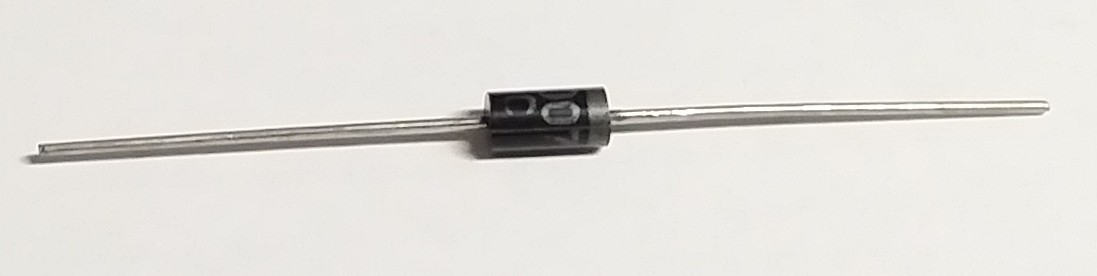
\includegraphics[width=0.75\linewidth]{./pics/diode.jpg}
%		
%%		\vspace{-1.5\baselineskip}
%		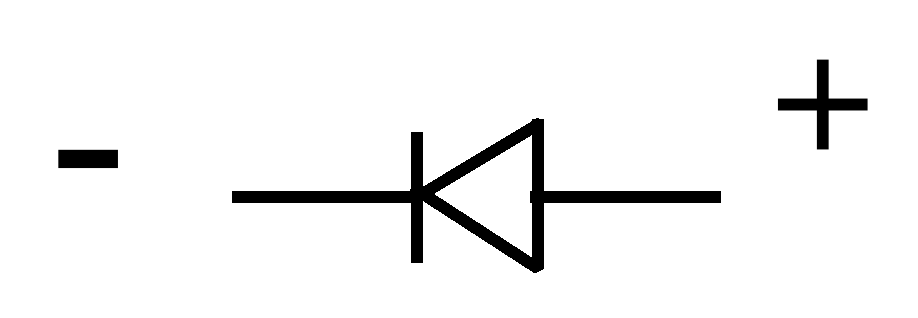
\includegraphics[width=0.75\linewidth,angle=180]{./Zeichnungen/diode-schaltsym.png}
%		\caption{Diode in real und als Schaltsymbol.}
%	\end{figure}
%\end{minipage}
%\medskip

Die Diode wird jedoch \emph{Sperrrichtung} eingebaut, also so, dass der Ring mit 5V und die andere Seite mit GND verbunden ist. Dadurch fließt im Normalbetrieb kein Strom durch die Diode. Wenn jedoch der entgegengerichtete Induktionsstrom des Motors auftritt, kann dieser durch die Diode abfließen, bis die verbleibende elektrische Energie vollständig in Wärme umgewandelt wurde.

\begin{recherche}{Verpolungsschutz}
	LEDs leuchten nicht, wenn man sie falsch herum anschließt. Andere Bauteile wie Elektrolytkondensatoren explodieren sogar, wenn man sie falsch herum anschließt. Um zu vermeiden, dass solche Schäden entstehen, wenn man eine Batterie falsch herum anschließt, werden in einigen Fällen Dioden genutzt. Recherchiere im \href{https://www.elektronik-kompendium.de/sites/slt/1206251.htm}{Elektronik-Kompendium},\footnote{\url{https://www.elektronik-kompendium.de/sites/slt/1206251.htm}} wie dies funktioniert.
\end{recherche}

\medskip
\begin{minipage}[t]{0.5\textwidth}
	\begin{aufgabe}
		Erkläre die Funktion der Diode parallel zum E-Motor in eigenen Worten.
		
		\smallskip
		Baue die rechts abgebildete Schaltung zum Betrieb eines Gleichstrom-Elektromotors am Arduino auf.
		
		\bigskip
		\ausrufezeichen \emph{Es ist sehr wichtig, dass die Diode richtig, also in Sperrrichtung, eingebaut wird, da sonst der Arduino zerstört werden könnte!}
	\end{aufgabe}
\end{minipage}
\hfill
\begin{minipage}[t]{0.48\textwidth}
	\begin{figure}[H]
		\centering
		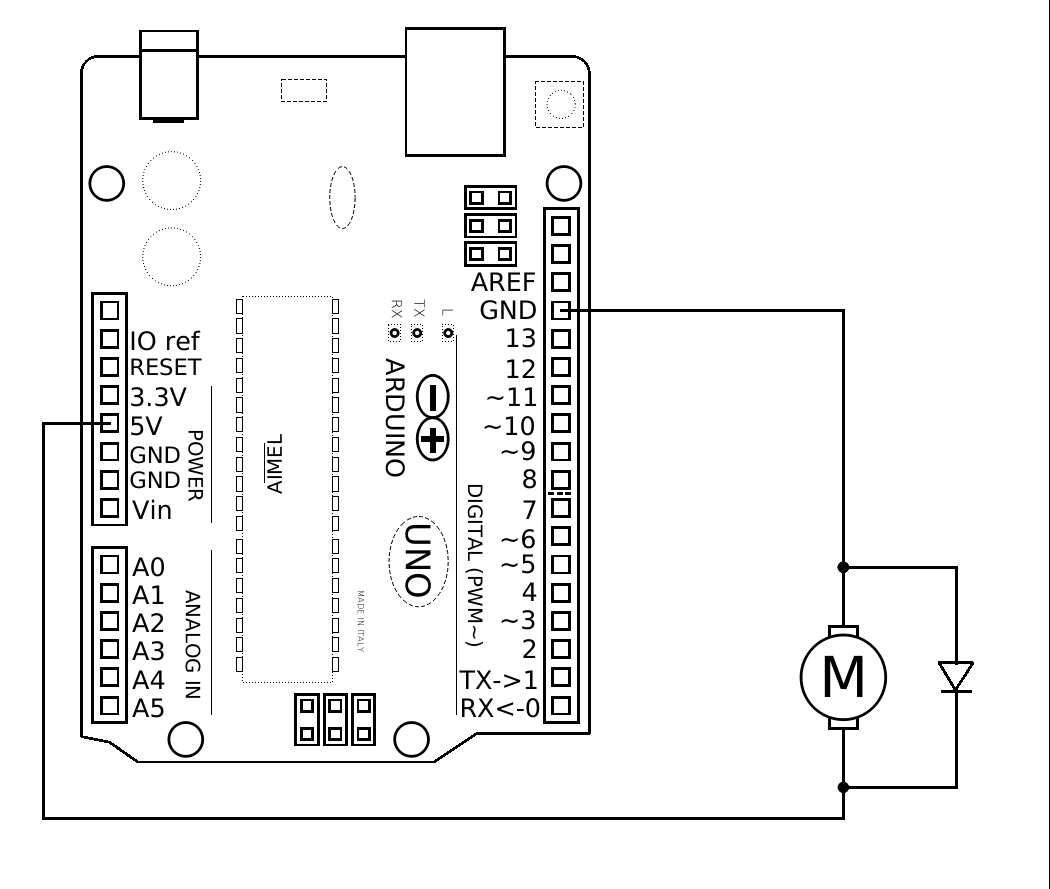
\includegraphics[width=0.9\textwidth]{./Zeichnungen/Schaltplan-Motoranschluss-einfach.png}
		\caption{Anschluss eines Gleichstrom-Elektromotors mit dem Arduino als Spannungsquelle.}
	\end{figure}
\end{minipage}
\medskip

\begin{recherche}{Aufbau von Gleichstrom-Elektromotoren}
	Oben wurde die Funktionsweise von Gleichstrom-Elektromotoren bereits angedeutet. Recherchiere im Internet den genauen Aufbau und Ablauf der Drehbewegung. 
\end{recherche}

\section{Steuerung mit Transistor}
% Steuerung mit Transistor

Der 5\,V-Pin des Arduino liefert zwar in vielen Fällen genügend Strom für den Motor, jedoch lässt er sich nicht programmieren. Dazu lässt sich ein Transistor einbauen.

\begin{ziel}
	\textbf{Frage:} Wie steuert man einen Elektromotor mit einem Transistor am Arduino?
\end{ziel}


\medskip
\begin{minipage}{0.5\textwidth}
	Die rechts abgebildete Schaltung zeigt, wie ein npn-Transistor eingebaut werden kann, um den Motor mithilfe von Digitalpin 9 zu schalten. Der Transistor lässt den Strom zwischen Emitter (E) und Kollektor (C) passieren, wenn die Spannung zwischen Basis (B) und Emitter (E) mehr als 0,7\,V beträgt, anderenfalls sperrt er. Der Vorwiderstand mit $R=\SI{1}{\kilo\ohm}$ sorgt dafür, dass der Basisstrom nicht zu groß wird.
	
	Es ist ratsam, die Basis mit einem PWM-Pin (gekennzeichnet durch $\sim$) zu verbinden, da sich dadurch die Geschwindigkeit des Motors steuern lässt.
\end{minipage}
\hfill
\begin{minipage}{0.48\textwidth}
	\begin{figure}[H]
		\centering
		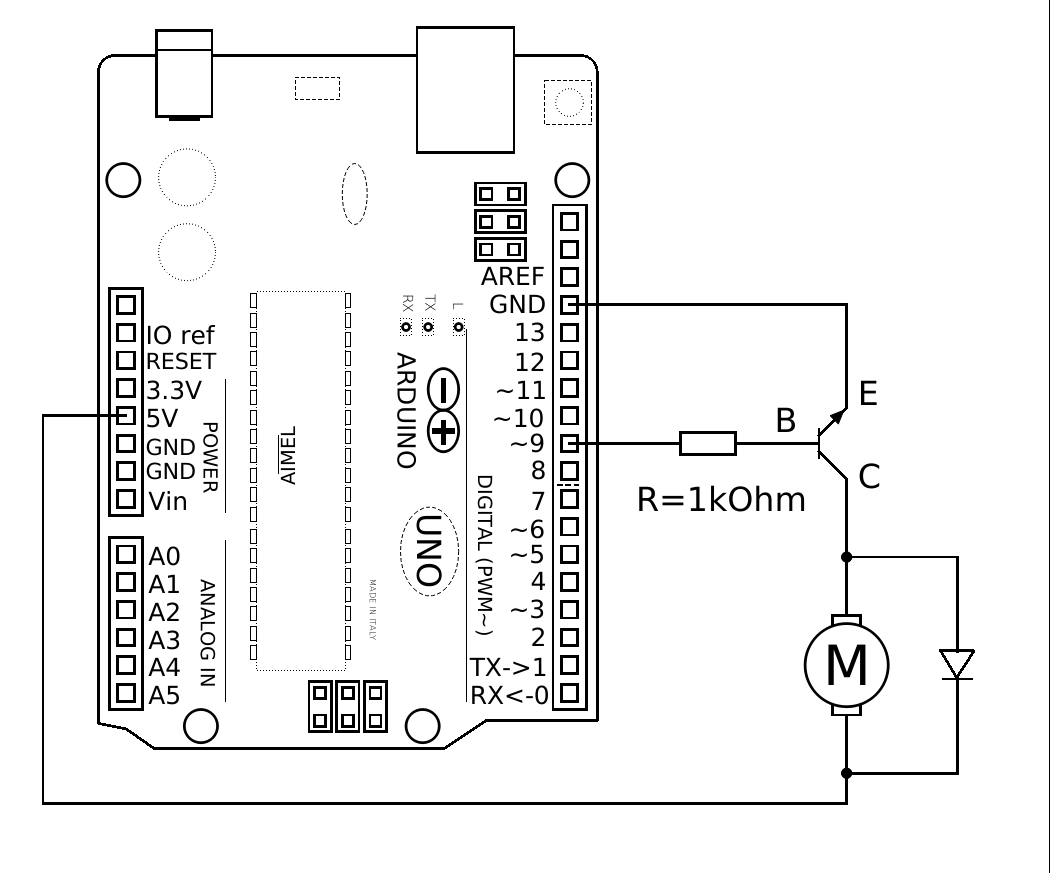
\includegraphics[width=\textwidth]{./Zeichnungen/Schaltplan-Motoranschluss-mit-Steuerung.png}
		\caption{Anschluss eines Gleichstrom-Elektromotors am Arduino mit Steuerung über einen Transistor an Digitalpin 9.}
	\end{figure}
\end{minipage}
\marginpar{%
	\scriptsize
	\centering
	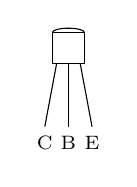
\begin{tikzpicture}
	\draw (-0.2,0.8) rectangle (0.2,1.2);
	\draw (0.2,1.2) arc [start angle=0,end angle=180,x radius=0.2,y radius=0.05];
	\draw (-0.15,0.8) -- (-0.3,0) node [below] {\scriptsize C};
	\draw (0,0.8) -- (0,0) node [below] {\scriptsize B};
	\draw (0.15,0.8) -- (0.3,0) node [below] {\scriptsize E};
	\end{tikzpicture}
	
	npn-Transistor; Blick auf flache Seite
}

\begin{aufgabe}
	
	Baue die oben abgebildete Schaltung auf und probiere die Steuerung des Motors mittels 
	
	\button{setze PWM-Pin <\_> auf <\_>} aus.
	
	Simuliere mit dem Motor eine konstant beschleunigende Bewegung (\emph{vgl. \href{sec:pwm}{Fading}}), gefolgt von einer abrupten Bremsung.
\end{aufgabe}

\begin{projekt}[Badezimmerlüfter]\label{proj:badezimmerluefter}
	Baue einen Badezimmerlüfter, der anspringt, wenn die Luftfeuchtigkeit größer als 65\% oder die Temperatur größer als $\SI{30}{\celsius}$ wird. Probiere deine Schaltung durch Anhauchen des Luftfeuchtigkeitssensors aus.
	
	\emph{Erweiterung:} Programmiere die Schaltung so, dass der Lüfter sich umso schneller dreht, je höher die Luftfeuchtigkeit ist.
\end{projekt}

\medskip
\emph{Schaltung mit externer Spannungsquelle}
\medskip

\begin{minipage}{0.5\textwidth}
	Wenn der verwendete Elektromotor größer ist und mehr Strom zieht bzw. größere Spannungen benötigt, muss für den Elektromotor eine eigene Spannungsquelle verwendet werden, die genügend Spannung und Strom bieten kann. Der rechts abgebildete Schaltplan zeigt, wie der Aufbau dann vorzunehmen ist. Wichtig ist dabei, dass ein gemeinsames GND-Niveau hergestellt wird - vergleichbar einem \enquote{Normalnull} für die Höhenangaben, hier allerdings als \enquote{Normalnull} für das elektrische Potenzial.
	
	Der Arduino kann über USB oder eine zweite Batterie mit Strom versorgt werden.
\end{minipage}
\hfill
\begin{minipage}{0.48\textwidth}
	\begin{figure}[H]
		\centering
		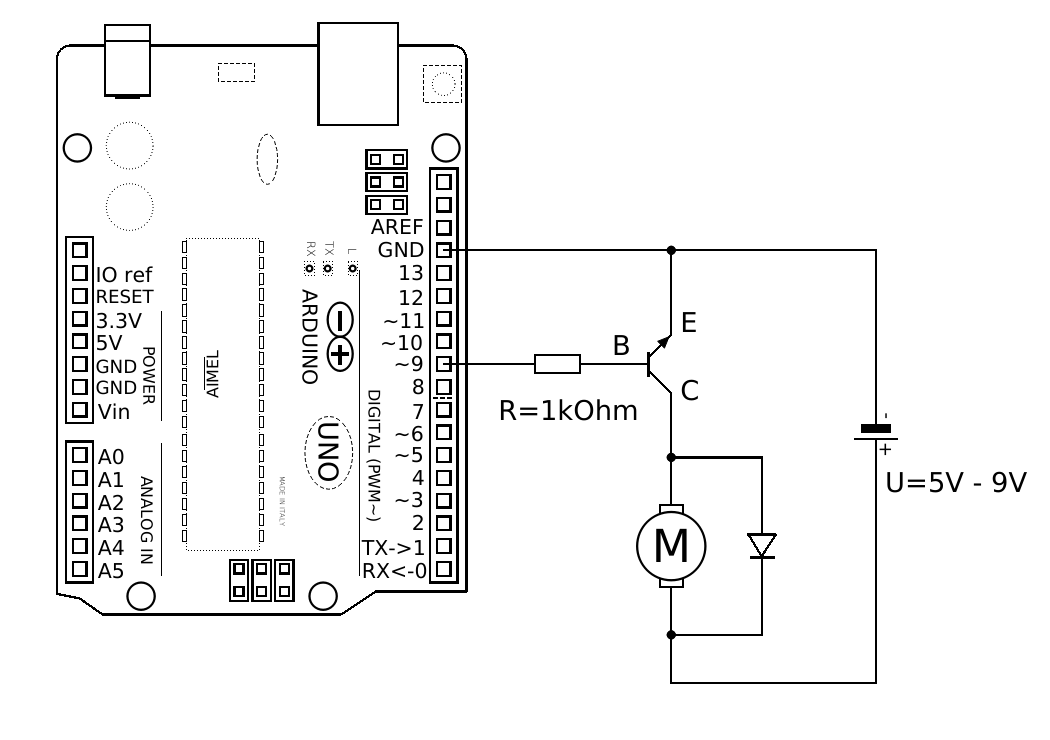
\includegraphics[width=\textwidth]{./Zeichnungen/Schaltplan-Motoranschluss-ext-Spannung.png}
		\caption{Anschluss eines Gleichstrom-Elektromotors am Arduino mit Steuerung über einen Transistor und mit externer Spannungsquelle für den Motor.}
	\end{figure}
\end{minipage}

\newpage
\section{Steuerung mit Relais}
% Steuerung von Motor mit Relais, Vgl zu Transistor-Schaltung

Wie oben zu sehen, muss der Arbeitsstromkreis mit dem Motor und der Steuerstromkreis mit dem Arduino bei Verwendung eines Transistors immer miteinander verbunden bleiben - auch bei sehr großen Stromstärken. Damit verbleibt immer eine gewisse Gefahr, dass eine Spannungsspitze auf den Arduino durchschlägt und ihn zerstört. Mit einem Relais lässt sich dieses Risiko vermeiden. Ein weiterer Vorteil ist, dass der Arbeitsstromkreis auch mit Wechselstrom betrieben werden kann, wenn ein Relais als Schalter genutzt wird.

\begin{ziel}
	\textbf{Frage:} Wie verwendet man ein Relais am Arduino?
\end{ziel}

Ein Relais (siehe unten, grau unterlegt) besteht im Wesentlichen aus einer Spule mit Eisenkern und einem Wechselschalter, an dem eine Feder angebracht ist.

\bigskip
% Aufbau Relais (mit Zeichnung für beide Zustände des Wechselschalters)
\begin{minipage}{0.48\textwidth}
	\begin{figure}[H]
		\centering
		%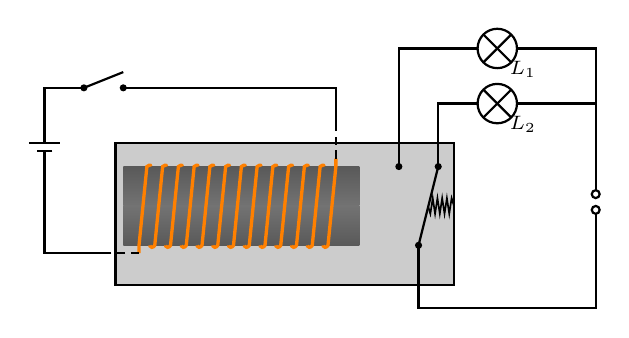
\begin{tikzpicture}
	% Kasten für Relais
	\draw [thick,fill=gray!40] (-0.1,-0.5) rectangle (4.2,1.3);
	%Eisenkern
	\shade [top color=gray!70!black, bottom color=gray!90!black] (0,0.5) rectangle (3,1);
	\shade [bottom color=gray!70!black, top color=gray!90!black] (0,0) rectangle (3,0.5);
	% Spule
	%Anfangspunkt (0.2,-0.1)
	\draw [color=orange, very thick] (0.2,-0.1) -- (0.2,0) -- ++(0.1,1) .. controls ++(0.05,0.04) and ++(0,0) .. ++(0.05,0);
	\foreach \x in {0.4,0.6,...,2.6} {
		\draw [color=orange, very thick] (\x-0.06,0) -- (\x-0.06,-0.01) .. controls ++(0.03,-0.04) and ++(0,0) .. (\x,0) -- ++(0.1,1) .. controls ++(0.05,0.04) and ++(0,0) .. ++(0.05,0);
	}
	\draw [color=orange, very thick] (2.6-0.06,0) -- (2.6-0.06,-0.01) .. controls ++(0.03,-0.04) and ++(0,0) .. (2.6,0) -- ++(0.1,1) -- ++(0,0.1);  % Endpunkt: (2.7,1.1)
	%%%% Steuerstromkreis
	\draw (2.7,1.1) [densely dashed, thick] -- (2.7,1.5);
	\draw [thick] (2.7,1.5) -- (2.7,2) -- (0,2);
	%Schalter offen
	\draw [thick,fill=black] (0,2) circle [radius=0.03]; 
	\draw [thick] (-0.5,2) -- ++ (0.5,0.2);
	\draw [thick,fill=black] (-0.5,2) circle [radius=0.03]; 
	\draw [thick] (-0.5,2) -- (-1,2) -- (-1,1.3) ++(-0.2,0) -- ++(0.4,0) ++(-0.1,-0.1) -- ++(-0.2,0) ++(0.1,0) -- (-1,-0.1) -- (-0.2,-0.1);
	\draw [thick,densely dashed] (0.2,-0.1) -- (-0.2,-0.1);
	%%%% Arbeitsstromkreis
	%Wechselschalter
	\draw [thick, fill=black] (3.75,0) circle [radius=0.03];
	\draw [thick, fill=black] (3.5,1) circle [radius=0.03];
	\draw [thick, fill=black] (4,1) circle [radius=0.03];
	\draw [thick] (3.75,0) -- (4,1);
	%Feder
	\draw [semithick] (4.2,0.5) -- ++(-0.03,0.1) -- ++(-0.03,-0.2) -- ++(-0.03,0.2) -- ++(-0.03,-0.2) -- ++(-0.03,0.2) -- ++(-0.03,-0.2)-- ++(-0.03,0.2) -- ++(-0.03,-0.2)-- ++(-0.03,0.2) -- ++(-0.03,-0.2) -- ++(-0.03,0.1);
	% Stromkreis an sich
	\draw [thick] (3.75,0) -- (3.75,-0.8) -- (6,-0.8) -- (6,0.4);
	\draw [thick] (6,0.45) circle [radius=0.05];
	\draw [thick] (4,1) -- (4,1.8) -- (4.5,1.8);
	\draw [thick] (4.75,1.8) circle [radius=0.25] node [below right =0.8] {\scriptsize $L_2$};
	\draw [thick] (4.75,1.8) -- ++(45:0.25);
	\draw [thick] (4.75,1.8) -- ++(135:0.25);
	\draw [thick] (4.75,1.8) -- ++(225:0.25);
	\draw [thick] (4.75,1.8) -- ++(315:0.25);
	\draw [thick] (5,1.8) -- (6,1.8) -- (6,0.7);
	\draw [thick] (6,0.65) circle [radius=0.05];
	\draw [thick] (3.5,1) -- (3.5,2.5) -- (4.5,2.5);
	\draw [thick] (4.75,2.5) circle [radius=0.25] node [below right =0.8] {\scriptsize $L_1$};
	\draw [thick] (4.75,2.5) -- ++(45:0.25);
	\draw [thick] (4.75,2.5) -- ++(135:0.25);
	\draw [thick] (4.75,2.5) -- ++(225:0.25);
	\draw [thick] (4.75,2.5) -- ++(315:0.25);
	\draw [thick] (5,2.5) -- (6,2.5) -- (6,1.8);
\end{tikzpicture}
		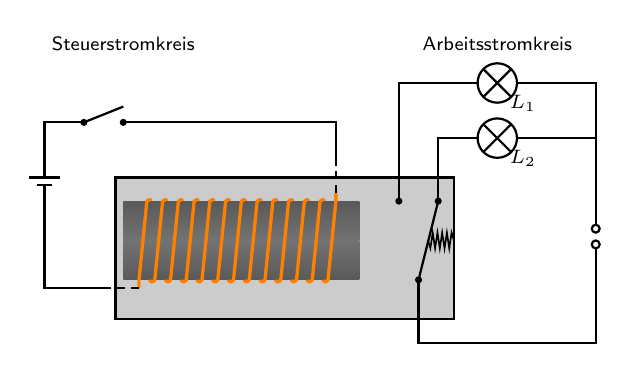
\begin{tikzpicture}
		% Kasten für Relais
		\draw [thick,fill=gray!40] (-0.1,-0.5) rectangle (4.2,1.3);
		%Eisenkern
		\shade [top color=gray!70!black, bottom color=gray!90!black] (0,0.5) rectangle (3,1);
		\shade [bottom color=gray!70!black, top color=gray!90!black] (0,0) rectangle (3,0.5);
		% Spule
		%Anfangspunkt (0.2,-0.1)
		\draw [color=orange, very thick] (0.2,-0.1) -- (0.2,0) -- ++(0.1,1) .. controls ++(0.05,0.04) and ++(0,0) .. ++(0.05,0);
		\foreach \x in {0.4,0.6,...,2.6} {
			\draw [color=orange, very thick] (\x-0.06,0) -- (\x-0.06,-0.01) .. controls ++(0.03,-0.04) and ++(0,0) .. (\x,0) -- ++(0.1,1) .. controls ++(0.05,0.04) and ++(0,0) .. ++(0.05,0);
		}
		\draw [color=orange, very thick] (2.6-0.06,0) -- (2.6-0.06,-0.01) .. controls ++(0.03,-0.04) and ++(0,0) .. (2.6,0) -- ++(0.1,1) -- ++(0,0.1);  % Endpunkt: (2.7,1.1)
		%%%% Steuerstromkreis
		\draw (2.7,1.1) [densely dashed, thick] -- (2.7,1.5);
		\draw [thick] (2.7,1.5) -- (2.7,2) -- (0,2);
		%Schalter offen
		\draw [thick,fill=black] (0,2) circle [radius=0.03]; 
		\draw [thick] (-0.5,2) -- ++ (0.5,0.2);
		\draw [thick,fill=black] (-0.5,2) circle [radius=0.03]; 
		\draw [thick] (-0.5,2) -- (-1,2) -- (-1,1.3) ++(-0.2,0) -- ++(0.4,0) ++(-0.1,-0.1) -- ++(-0.2,0) ++(0.1,0) -- (-1,-0.1) -- (-0.2,-0.1);
		\draw [thick,densely dashed] (0.2,-0.1) -- (-0.2,-0.1);
		%%%% Arbeitsstromkreis
		%Wechselschalter
		\draw [thick, fill=black] (3.75,0) circle [radius=0.03];
		\draw [thick, fill=black] (3.5,1) circle [radius=0.03];
		\draw [thick, fill=black] (4,1) circle [radius=0.03];
		\draw [thick] (3.75,0) -- (4,1);
		%Feder
		\draw [semithick] (4.2,0.5) -- ++(-0.03,0.1) -- ++(-0.03,-0.2) -- ++(-0.03,0.2) -- ++(-0.03,-0.2) -- ++(-0.03,0.2) -- ++(-0.03,-0.2)-- ++(-0.03,0.2) -- ++(-0.03,-0.2)-- ++(-0.03,0.2) -- ++(-0.03,-0.2) -- ++(-0.03,0.1);
		% Stromkreis an sich
		\draw [thick] (3.75,0) -- (3.75,-0.8) -- (6,-0.8) -- (6,0.4);
		\draw [thick] (6,0.45) circle [radius=0.05];
		\draw [thick] (4,1) -- (4,1.8) -- (4.5,1.8);
		\draw [thick] (4.75,1.8) circle [radius=0.25] node [below right =0.8] {\scriptsize\sffamily $L_2$};
		\draw [thick] (4.75,1.8) -- ++(45:0.25);
		\draw [thick] (4.75,1.8) -- ++(135:0.25);
		\draw [thick] (4.75,1.8) -- ++(225:0.25);
		\draw [thick] (4.75,1.8) -- ++(315:0.25);
		\draw [thick] (5,1.8) -- (6,1.8) -- (6,0.7);
		\draw [thick] (6,0.65) circle [radius=0.05];
		\draw [thick] (3.5,1) -- (3.5,2.5) -- (4.5,2.5);
		\draw [thick] (4.75,2.5) circle [radius=0.25] node [below right =0.8] {\scriptsize\sffamily $L_1$};
		\draw [thick] (4.75,2.5) -- ++(45:0.25);
		\draw [thick] (4.75,2.5) -- ++(135:0.25);
		\draw [thick] (4.75,2.5) -- ++(225:0.25);
		\draw [thick] (4.75,2.5) -- ++(315:0.25);
		\draw [thick] (5,2.5) -- (6,2.5) -- (6,1.8);
		% Bezeichnungen
		\node at (0,3) {\scriptsize\sffamily Steuerstromkreis};
		\node at (4.75,3) {\scriptsize\sffamily Arbeitsstromkreis};
		\end{tikzpicture}
		\caption{Aufbau eines Relais (grau unterlegt) einschließlich der Stellung des Wechselschalters, wenn im Steuerstromkreis kein Strom fließt.}
	\end{figure}
\end{minipage}
\hfill
\begin{minipage}{0.48\textwidth}
	\begin{figure}[H]
		\centering
		%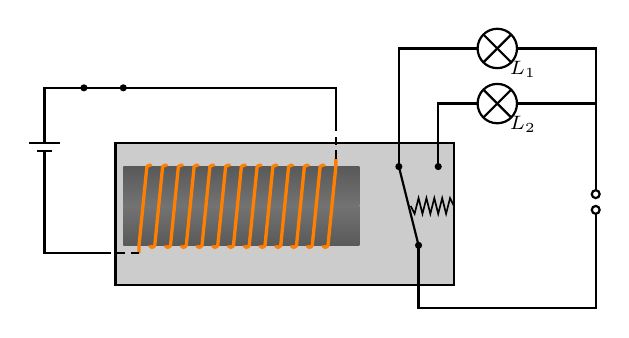
\begin{tikzpicture}
	% Kasten für Relais
	\draw [thick,fill=gray!40] (-0.1,-0.5) rectangle (4.2,1.3);
	%Eisenkern
	\shade [top color=gray!70!black, bottom color=gray!90!black] (0,0.5) rectangle (3,1);
	\shade [bottom color=gray!70!black, top color=gray!90!black] (0,0) rectangle (3,0.5);
	% Spule
	%Anfangspunkt (0.2,-0.1)
	\draw [color=orange, very thick] (0.2,-0.1) -- (0.2,0) -- ++(0.1,1) .. controls ++(0.05,0.04) and ++(0,0) .. ++(0.05,0);
	\foreach \x in {0.4,0.6,...,2.6} {
		\draw [color=orange, very thick] (\x-0.06,0) -- (\x-0.06,-0.01) .. controls ++(0.03,-0.04) and ++(0,0) .. (\x,0) -- ++(0.1,1) .. controls ++(0.05,0.04) and ++(0,0) .. ++(0.05,0);
	}
	\draw [color=orange, very thick] (2.6-0.06,0) -- (2.6-0.06,-0.01) .. controls ++(0.03,-0.04) and ++(0,0) .. (2.6,0) -- ++(0.1,1) -- ++(0,0.1);  % Endpunkt: (2.7,1.1)
	%%%% Steuerstromkreis
	\draw (2.7,1.1) [densely dashed, thick] -- (2.7,1.5);
	\draw [thick] (2.7,1.5) -- (2.7,2) -- (0,2);
	%Schalter geschlossen
	\draw [thick,fill=black] (0,2) circle [radius=0.03]; 
	\draw [thick] (-0.5,2) -- ++ (0.5,0);
	\draw [thick,fill=black] (-0.5,2) circle [radius=0.03]; 
	\draw [thick] (-0.5,2) -- (-1,2) -- (-1,1.3) ++(-0.2,0) -- ++(0.4,0) ++(-0.1,-0.1) -- ++(-0.2,0) ++(0.1,0) -- (-1,-0.1) -- (-0.2,-0.1);
	\draw [thick,densely dashed] (0.2,-0.1) -- (-0.2,-0.1);
	%%%% Arbeitsstromkreis
	%Wechselschalter
	\draw [thick, fill=black] (3.75,0) circle [radius=0.03];
	\draw [thick, fill=black] (3.5,1) circle [radius=0.03];
	\draw [thick, fill=black] (4,1) circle [radius=0.03];
	\draw [thick] (3.75,0) -- (3.5,1);
	%Feder
	\draw [semithick] (4.2,0.5) -- ++(-0.05,0.1) -- ++(-0.05,-0.2) -- ++(-0.05,0.2) -- ++(-0.05,-0.2) -- ++(-0.05,0.2) -- ++(-0.05,-0.2)-- ++(-0.05,0.2) -- ++(-0.05,-0.2)-- ++(-0.05,0.2) -- ++(-0.05,-0.2) -- ++(-0.05,0.1);
	% Stromkreis an sich
	\draw [thick] (3.75,0) -- (3.75,-0.8) -- (6,-0.8) -- (6,0.4);
	\draw [thick] (6,0.45) circle [radius=0.05];
	\draw [thick] (4,1) -- (4,1.8) -- (4.5,1.8);
	%Lampe L2
	\draw [thick] (4.75,1.8) circle [radius=0.25] node [below right =0.8] {\scriptsize $L_2$};
	\draw [thick] (4.75,1.8) -- ++(45:0.25);
	\draw [thick] (4.75,1.8) -- ++(135:0.25);
	\draw [thick] (4.75,1.8) -- ++(225:0.25);
	\draw [thick] (4.75,1.8) -- ++(315:0.25);
	%weiter mit Kabels
	\draw [thick] (5,1.8) -- (6,1.8) -- (6,0.7);
	\draw [thick] (6,0.65) circle [radius=0.05];
	\draw [thick] (3.5,1) -- (3.5,2.5) -- (4.5,2.5);
	%Lampe L1
	\draw [thick] (4.75,2.5) circle [radius=0.25] node [below right =0.8] {\scriptsize $L_1$};
	\draw [thick] (4.75,2.5) -- ++(45:0.25);
	\draw [thick] (4.75,2.5) -- ++(135:0.25);
	\draw [thick] (4.75,2.5) -- ++(225:0.25);
	\draw [thick] (4.75,2.5) -- ++(315:0.25);
	% Kabels
	\draw [thick] (5,2.5) -- (6,2.5) -- (6,1.8);
\end{tikzpicture}
		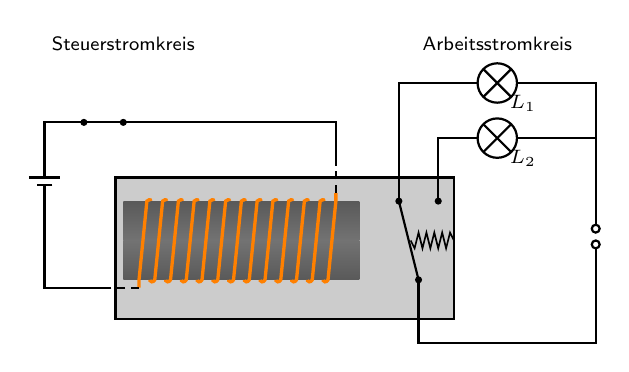
\begin{tikzpicture}
		% Kasten für Relais
		\draw [thick,fill=gray!40] (-0.1,-0.5) rectangle (4.2,1.3);
		%Eisenkern
		\shade [top color=gray!70!black, bottom color=gray!90!black] (0,0.5) rectangle (3,1);
		\shade [bottom color=gray!70!black, top color=gray!90!black] (0,0) rectangle (3,0.5);
		% Spule
		%Anfangspunkt (0.2,-0.1)
		\draw [color=orange, very thick] (0.2,-0.1) -- (0.2,0) -- ++(0.1,1) .. controls ++(0.05,0.04) and ++(0,0) .. ++(0.05,0);
		\foreach \x in {0.4,0.6,...,2.6} {
			\draw [color=orange, very thick] (\x-0.06,0) -- (\x-0.06,-0.01) .. controls ++(0.03,-0.04) and ++(0,0) .. (\x,0) -- ++(0.1,1) .. controls ++(0.05,0.04) and ++(0,0) .. ++(0.05,0);
		}
		\draw [color=orange, very thick] (2.6-0.06,0) -- (2.6-0.06,-0.01) .. controls ++(0.03,-0.04) and ++(0,0) .. (2.6,0) -- ++(0.1,1) -- ++(0,0.1);  % Endpunkt: (2.7,1.1)
		%%%% Steuerstromkreis
		\draw (2.7,1.1) [densely dashed, thick] -- (2.7,1.5);
		\draw [thick] (2.7,1.5) -- (2.7,2) -- (0,2);
		%Schalter geschlossen
		\draw [thick,fill=black] (0,2) circle [radius=0.03]; 
		\draw [thick] (-0.5,2) -- ++ (0.5,0);
		\draw [thick,fill=black] (-0.5,2) circle [radius=0.03]; 
		\draw [thick] (-0.5,2) -- (-1,2) -- (-1,1.3) ++(-0.2,0) -- ++(0.4,0) ++(-0.1,-0.1) -- ++(-0.2,0) ++(0.1,0) -- (-1,-0.1) -- (-0.2,-0.1);
		\draw [thick,densely dashed] (0.2,-0.1) -- (-0.2,-0.1);
		%%%% Arbeitsstromkreis
		%Wechselschalter
		\draw [thick, fill=black] (3.75,0) circle [radius=0.03];
		\draw [thick, fill=black] (3.5,1) circle [radius=0.03];
		\draw [thick, fill=black] (4,1) circle [radius=0.03];
		\draw [thick] (3.75,0) -- (3.5,1);
		%Feder
		\draw [semithick] (4.2,0.5) -- ++(-0.05,0.1) -- ++(-0.05,-0.2) -- ++(-0.05,0.2) -- ++(-0.05,-0.2) -- ++(-0.05,0.2) -- ++(-0.05,-0.2)-- ++(-0.05,0.2) -- ++(-0.05,-0.2)-- ++(-0.05,0.2) -- ++(-0.05,-0.2) -- ++(-0.05,0.1);
		% Stromkreis an sich
		\draw [thick] (3.75,0) -- (3.75,-0.8) -- (6,-0.8) -- (6,0.4);
		\draw [thick] (6,0.45) circle [radius=0.05];
		\draw [thick] (4,1) -- (4,1.8) -- (4.5,1.8);
		%Lampe L2
		\draw [thick] (4.75,1.8) circle [radius=0.25] node [below right =0.8] {\scriptsize\sffamily $L_2$};
		\draw [thick] (4.75,1.8) -- ++(45:0.25);
		\draw [thick] (4.75,1.8) -- ++(135:0.25);
		\draw [thick] (4.75,1.8) -- ++(225:0.25);
		\draw [thick] (4.75,1.8) -- ++(315:0.25);
		%weiter mit Kabels
		\draw [thick] (5,1.8) -- (6,1.8) -- (6,0.7);
		\draw [thick] (6,0.65) circle [radius=0.05];
		\draw [thick] (3.5,1) -- (3.5,2.5) -- (4.5,2.5);
		%Lampe L1
		\draw [thick] (4.75,2.5) circle [radius=0.25] node [below right =0.8] {\scriptsize\sffamily $L_1$};
		\draw [thick] (4.75,2.5) -- ++(45:0.25);
		\draw [thick] (4.75,2.5) -- ++(135:0.25);
		\draw [thick] (4.75,2.5) -- ++(225:0.25);
		\draw [thick] (4.75,2.5) -- ++(315:0.25);
		% Kabels
		\draw [thick] (5,2.5) -- (6,2.5) -- (6,1.8);
		% Bezeichnungen
		\node at (0,3) {\scriptsize\sffamily Steuerstromkreis};
		\node at (4.75,3) {\scriptsize\sffamily Arbeitsstromkreis};
		\end{tikzpicture}
		\caption{Aufbau eines Relais (grau unterlegt) einschließlich der Stellung des Wechselschalters, wenn im Steuerstromkreis Strom fließt.}
	\end{figure}
\end{minipage}

\bigskip
\begin{aufgabe}\emph{Physikalischer Hintergrund zum Relais}
	
	Erkläre die Stellung des Wechselschalters in Abhängigkeit des Steuerstromkreises in den beiden abgebildeten Situationen. Welche Lampe leuchtet?
	
	Die Kontakte am Wechselschalter werden mit \emph{NO} (\emph{normally open}), \emph{NC} (\emph{normally closed}) und \emph{C} (\emph{common ground}) bezeichnet. Ordne die Bezeichnungen den Kontakten in der Skizze zu.
\end{aufgabe}

\begin{aufgabe}\emph{Anschluss eines Relais}
	
	\begin{wrapfigure}{r}{0.3\textwidth}
		\vspace{-\baselineskip}
		\centering
		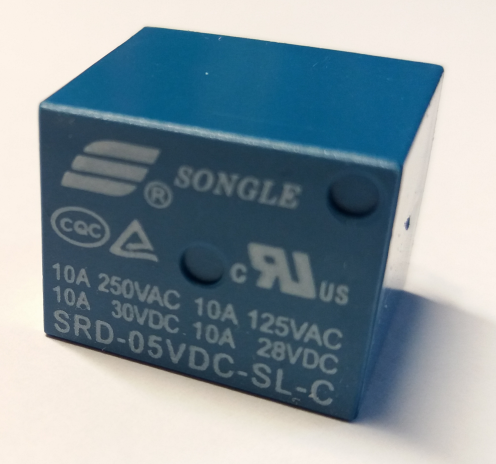
\includegraphics[width=0.17\textwidth]{./pics/relais-klein.png}
	\end{wrapfigure}
	\textbf{a)} Wie aus dem obigen Schaltplan ersichtlich wird, hat ein Relais fünf Anschlüsse, die jedoch nicht beschriftet sind. Suche im Internet nach \enquote{Datasheet <Gerätebezeichnung des Relais>} (Bezeichnung vom Relais ablesen) und entnimm dem Datenblatt, welche Anschlüsse zum Steuer- bzw. Arbeitsstromkreis gehören.
	
	\medskip
	\ausrufezeichen \textbf{Achtung:} Auf dem Relais ist angegeben, dass damit bis zu $\SI{250}{\volt}$ Wechselspannung und $\SI{10}{\ampere}$ geschaltet werden können. Das sollte man mit solch billigen Bastelmodulen aber \textbf{niemals machen}! Generell gilt: \textbf{Nur ausgebildete Fachleute sollten mit Spannungen von mehr als 24\,V hantieren!}
	
	\bigskip
	\begin{minipage}{0.44\textwidth}
		\textbf{b)} Baue die Schaltung entsprechend des rechts abgebildeten Schaltplans auf. Nutze dazu das \enquote{Power Module} auf dem Steckbrett (Erklärung unten). Probiere die Schaltung des Relais aus, indem du die Stromzufuhr der Spule unterbrichst und wieder herstellst.
	\end{minipage}
	\hfill
	\begin{minipage}{0.54\textwidth}
		\centering
		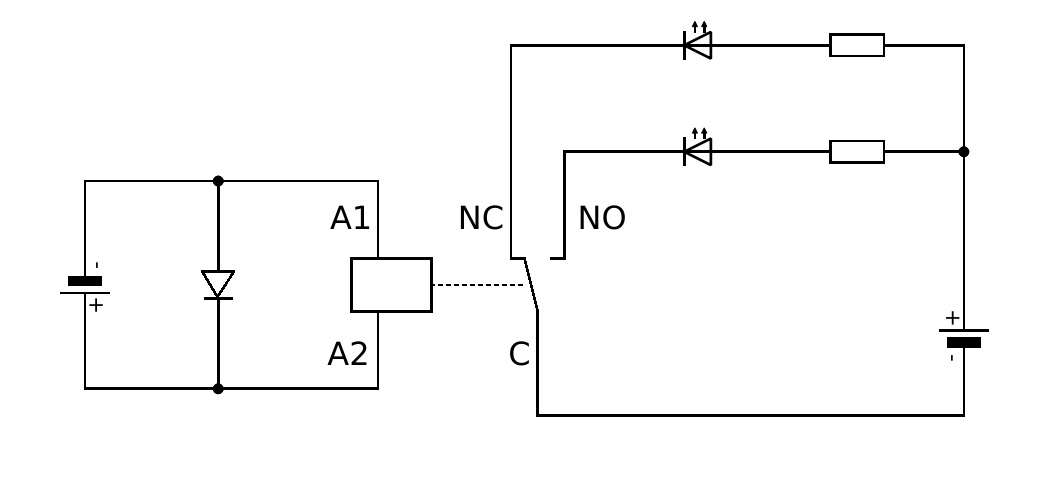
\includegraphics[width=\textwidth]{./Zeichnungen/relais-schaltung-ohne-arduino.png}
	\end{minipage}
	
	\medskip
	\textbf{c)} Ordne in einer Skizze des Relais die Anschlüsse ihrer Bezeichnung (A1, A2, C, NO, NC) zu.
\end{aufgabe}
% Erklärung der Pins des Relais + Ausprobieren der NC-Verbindung und NO-Verbindung mit LED+Vorwiderstand -> in Skizze festhalten, wo NC und wo NO ist

\bigskip
\begin{zsfg}{Das \enquote{Power Supply Module}}\label{powersupplymodule}
	
	\begin{wrapfigure}{r}{0.37\textwidth}
		\vspace{-0.5\baselineskip}
		\centering
		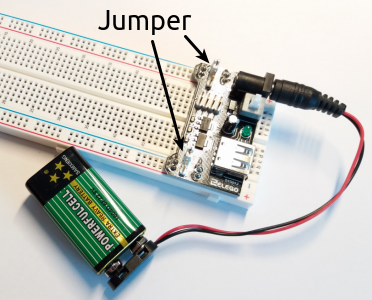
\includegraphics[width=0.35\textwidth]{./pics/steckbrett-mit-power-module-klein.png}
		\vspace{-\baselineskip}
	\end{wrapfigure}
	Das Power Supply Module dient zur Spannungsversorgung auf einem Steckbrett. Dazu kann eine Batterie mit $\SI{6,5}{\volt}$ bis $\SI{12}{\volt}$ oder ein USB-Kabel angeschlossen werden. Die Spannung wird auf dem Modul je nach Einstellung der \emph{Jumper} auf $\SI{5}{\volt}$ oder $\SI{3,3}{\volt}$ heruntergeregelt. Dazu verbindet man mithilfe der Jumper die Anschlüsse \texttt{5V} und \texttt{OFF} bzw. \texttt{3.3} und \texttt{OFF}.
	
	Die Spannung kann entlang der langen äußeren Leisten abgegriffen werden, wenn der Taster neben der Hohlbuchse gedrückt ist. Die Zuordnung zu Pluspol und Minuspol ist auf dem Power Supply Module mit \texttt{+} bzw. \texttt{-} markiert.
\end{zsfg}
% Gefahrenhinweis!
% Erklärung des Steuerstromkreises mit Transistor und Diode
% Aufgabe: Aufbauen und ausprobieren

\begin{aufgabe}\emph{Anschluss eines Relais am Arduino}
	\vspace{-0.5\baselineskip}
	\begin{figure}[H]
		\centering
		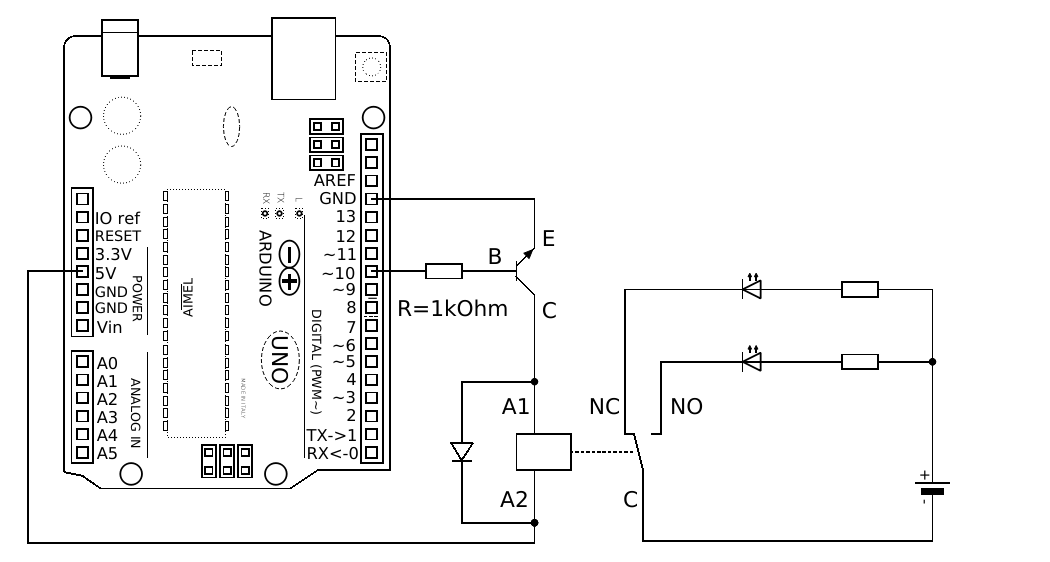
\includegraphics[width=0.65\textwidth]{./Zeichnungen/relais-schaltung-mit-arduino.png}
	\end{figure}
	\vspace{-0.5\baselineskip}
	\marginpar{%
		\scriptsize
		\centering
		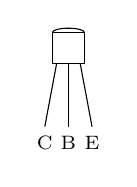
\begin{tikzpicture}
		\draw (-0.2,0.8) rectangle (0.2,1.2);
		\draw (0.2,1.2) arc [start angle=0,end angle=180,x radius=0.2,y radius=0.05];
		\draw (-0.15,0.8) -- (-0.3,0) node [below] {\scriptsize C};
		\draw (0,0.8) -- (0,0) node [below] {\scriptsize B};
		\draw (0.15,0.8) -- (0.3,0) node [below] {\scriptsize E};
		\end{tikzpicture}
		
		npn-Transistor; Blick auf flache Seite
	}
	Der Schaltplan oben zeigt, wie man ein Relais mit dem Arduino steuert.
	\begin{enumerate}[itemsep=0mm, parsep=0mm, label=\alph*)]
		\item Erkläre die Funktion der in Sperrrichtung geschalteten Diode parallel zur Spule des Relais.
		\item Erkläre die Funktion des Transistors.
		
		\emph{Hinweis:} Der 5V-Pin und der GND-Pin vertragen bis zu $\SI{200}{\milli\ampere}$. Die Digitalpins vertragen dagegen maximal $\SI{40}{\milli\ampere}$; normalerweise sollten $\SI{20}{\milli\ampere}$ nicht überschritten werden (s. \href{https://playground.arduino.cc/Main/ArduinoPinCurrentLimitations/}{Pin Current Limitations}).
		\item Baue die Schaltung auf und teste sie mit einem Blink-Programm.
	\end{enumerate}
\end{aufgabe}

% E-Motor anschließen
\begin{projekt}[Waschmaschinensteuerung]\label{proj:waschmaschinensteuerung}
	\begin{figure}[H]
		\centering
		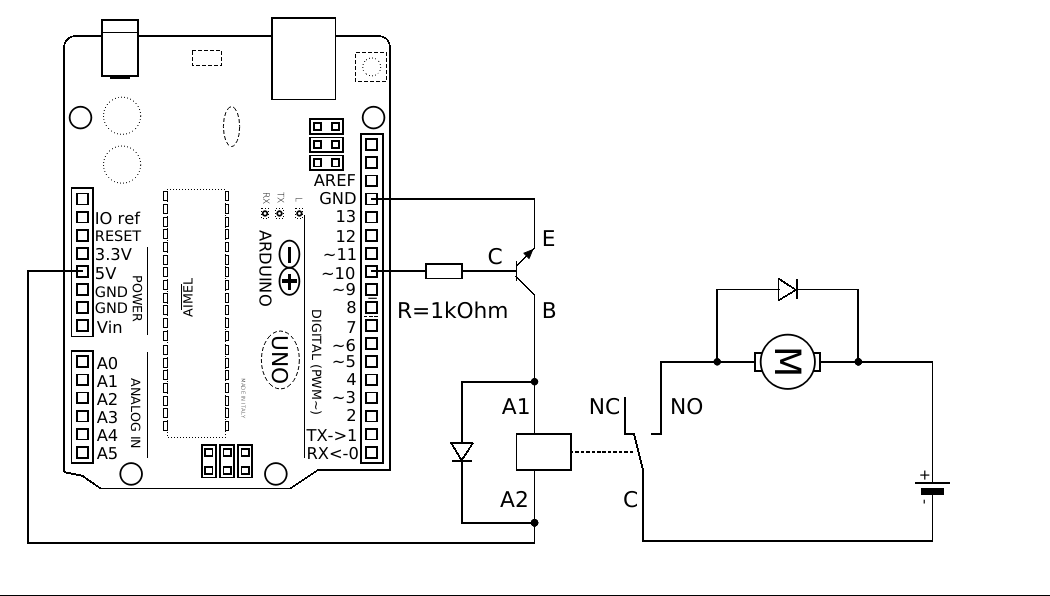
\includegraphics[width=0.7\textwidth]{./Zeichnungen/relais-schaltung-mit-motor.png}
	\end{figure}
	Baue die oben abgebildete Schaltung zur Steuerung eines Elektromotors mit einem Relais am Arduino auf. Achte auf die in Sperrrichtung geschaltete Diode parallel zum Motor.
	
	Schließe dann drei Taster an (mit Widerstand! - vgl. Abschnitt \ref{sec:taster}).
	
	\emph{Programmiere nun einen einfachen steuerbaren Waschmaschinenprototypen!}
	
	Dieser gibt solange auf dem seriellen Monitor die aktuell gesetzte Waschzeit aus, bis der mittlere Taster gedrückt wurde, was bedeutet, dass der Waschvorgang startet (der Motor dreht sich für die angegebene Zeit). Wenn der linke Taster gedrückt wird, wird die Waschzeit verringert (aber nicht niedriger als eine Sekunde). Wenn der rechte Taster gedrückt wird, wird die Waschzeit vergrößert (aber nicht größer als 30 Sekunden). Nach dem Waschen fragt der Waschmaschinenprototyp wieder nach der Waschzeit.
\end{projekt}

\begin{recherche}{Anwendungen von Relais}
	Recherchiere einige Anwendungen von Relais. Einen guten Startpunkt bietet die \href{https://www.leifiphysik.de/elektrizitaetslehre/elektromagnetismus/ausblick/relais}{Seite von Leifiphysik}.
\end{recherche}
% Recherchiere Anwendungen von Relais-Schaltungen, z. B. bei Leifiphysik

\begin{aufgabe} \emph{Vergleich von Transistor und Relais}
	
	Transistoren und Relais erfüllen im Wesentlichen die gleiche Funktion: Sie sind elektronisch steuerbare Schalter, bei denen die zu steuernde Stromstärke größer sein kann als die Stromstärke im Steuerstromkreis. Dennoch gibt es einige Unterschiede, weshalb sie für unterschiedliche Aufgaben geeignet sind.
	
	Vergleiche die Steuerung mit einem Transistor und mit einem Relais hinsichtlich der Vor- und Nachteile.
\end{aufgabe}
% Vergleiche die Steuerung mit einem Transistor und mit einem Relais im Hinblick auf die jeweiligen Vor- und Nachteile.

\newpage
\section{Steuerung mit dem Motortreiber-IC L293D (inkl. Drehrichtung)}

Die Steuerung von Motoren erfordert in den oben beschriebenen Fällen stets mehrere Bauteile und einige Überlegungen zum Aufbau der Schaltung. Außerdem kann dabei nicht die Drehrichtung geändert werden. Der integrierte Schaltkreis L293D vereinfacht den Aufbau der Schaltung für gleich zwei Motoren und ermöglicht zusätzlich die flexible Steuerung der Drehrichtung.

\begin{ziel}
	\textbf{Frage:} Wie steuert man einen Motor mit dem L293D? 
\end{ziel}

% Aufbau des IC - Vierquadrantensteller
\begin{aufgabe} \emph{Aufbau des L293D - der Vierquadrantensteller}
	
	Um die Drehrichtung des Motors kontrollieren zu können, braucht man eine spezielle Anordnung von Transistoren, die als \emph{H-Brücke} oder \emph{Vierquadrantensteller} bezeichnet wird. Dieser Aufbau befindet sich auch im L293D.
	
	\begin{figure}[H]
		\centering
		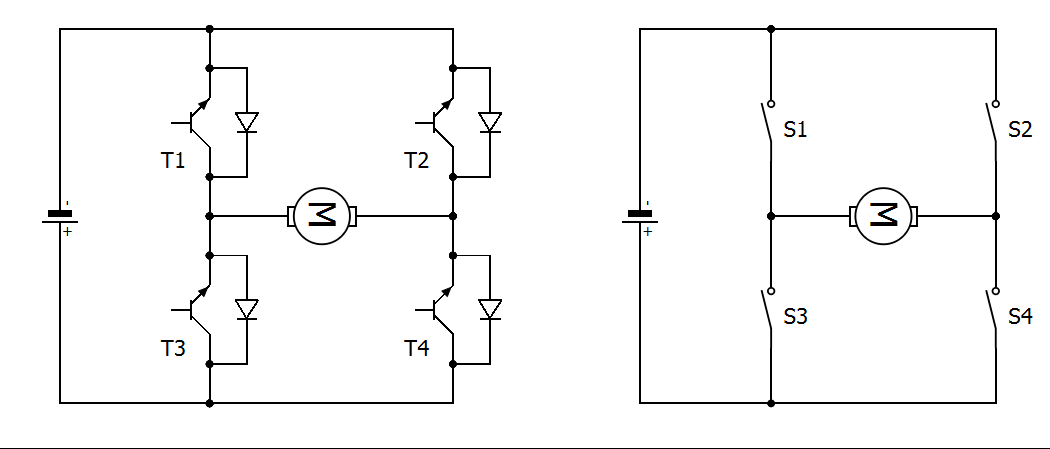
\includegraphics[width=0.8\textwidth]{./Zeichnungen/vierquadrantensteller.png}
		\caption{Vereinfachter Aufbau eines Vierquadrantenstellers mit Transistoren und zugehörigen Freilaufdioden (links) sowie die noch einmal vereinfachte Ersatzschaltung mit Schaltern.}
	\end{figure}

	\begin{enumerate}[label=\alph*), itemsep=0mm, parsep=0mm]
		\item Die Drehrichtung des Motors hängt davon ab, in welcher Richtung der Strom durch den Motor fließt. Notiere, welche Transistoren\,/\,Schalter eingeschaltet und welche Transistoren\,/\,Schalter ausgeschaltet sein müssen, damit der Strom von links nach rechts durch den Motor fließt. Notiere danach die Kombination für die Stromrichtung von rechts nach links.
		\item Erkläre, wie sich der Motor mithilfe der vier Transistoren bzw. Schalter bremsen lässt.
		\item Welche Schaltkombinationen der Transistoren müssen unbedingt vermieden werden?
	\end{enumerate}

	\emph{Hinweis:} Die Freilaufdioden dienen dazu, die vom Motor induzierten Ströme abfließen zu lassen.
\end{aufgabe}

Da stets zwei Transistoren gemeinsam eingeschaltet werden müssen, könnten diese beim Anschluss an den Arduino über einen gemeinsamen Digitalpin gesteuert werden. Zudem ist es im Allgemeinen sinnvoll, für den Motor und den Arduino verschiedene Spannungsquellen zu verwenden, die über einen gemeinsamen GND-Anschluss geerdet werden, damit die möglicherweise hohen Ströme des Motors den Arduino nicht zerstören.

\begin{figure}[H]
	\centering
	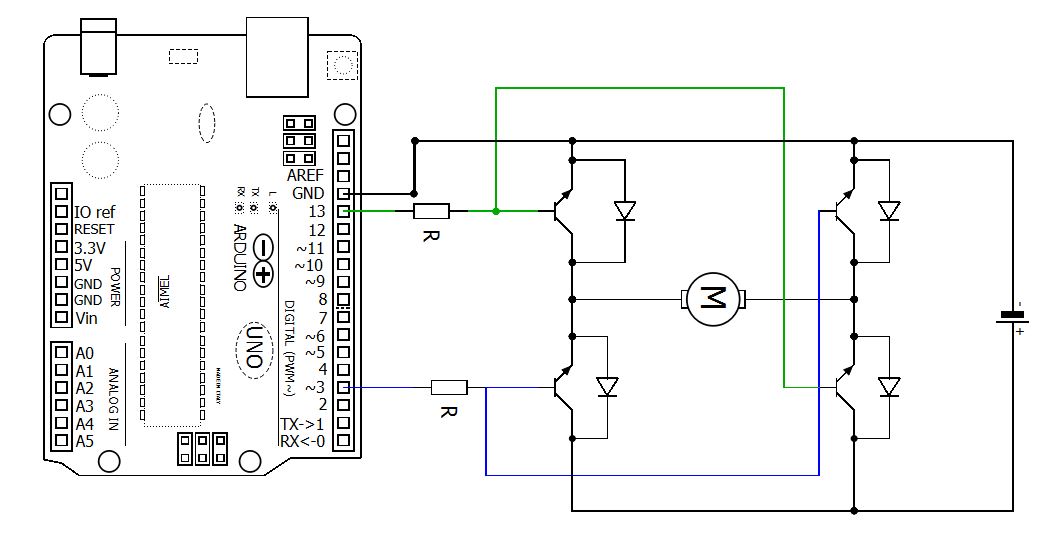
\includegraphics[width=0.8\textwidth]{./Zeichnungen/vierquadrantensteller-an-arduino.png}
	\caption{Steuerung eines Motors mit einem Vierquadrantensteller am Arduino.}
\end{figure}

Bei der oben dargestellten Schaltung muss jedoch immer noch genau darauf geachtet werden, dass nicht versehentlich alle vier Transitoren leitend geschaltet werden. Daher ist die Steuerung mit dem L293D noch ein wenig komplexer - die oben angestellten Überlegungen verdeutlichen aber gut den prinzipiellen Aufbau.

\begin{zsfg}{Der Motortreiber L293D}
	
	\medskip
	\begin{minipage}{0.7\textwidth}
		Der L293D ist ein integrierter Schaltkreis (\emph{IC} von engl. \emph{integrated circuit}), das heißt, in das schwarze Gehäuse sind Schaltkreise mit Transistoren, Widerständen, Dioden etc. integriert. Genauer gesagt, enthält der L293D zwei H-Brücken oder Vierquadrantensteller, die sich mit den Pins an beiden Seiten steuern lassen. Bei der Nummerierung der Pins ist darauf zu achten, dass die kleine Kerbe nach oben gehalten wird.
	\end{minipage}
	\hfill
	\begin{minipage}{0.28\textwidth}
		\begin{minipage}{0.48\textwidth}
			\centering
			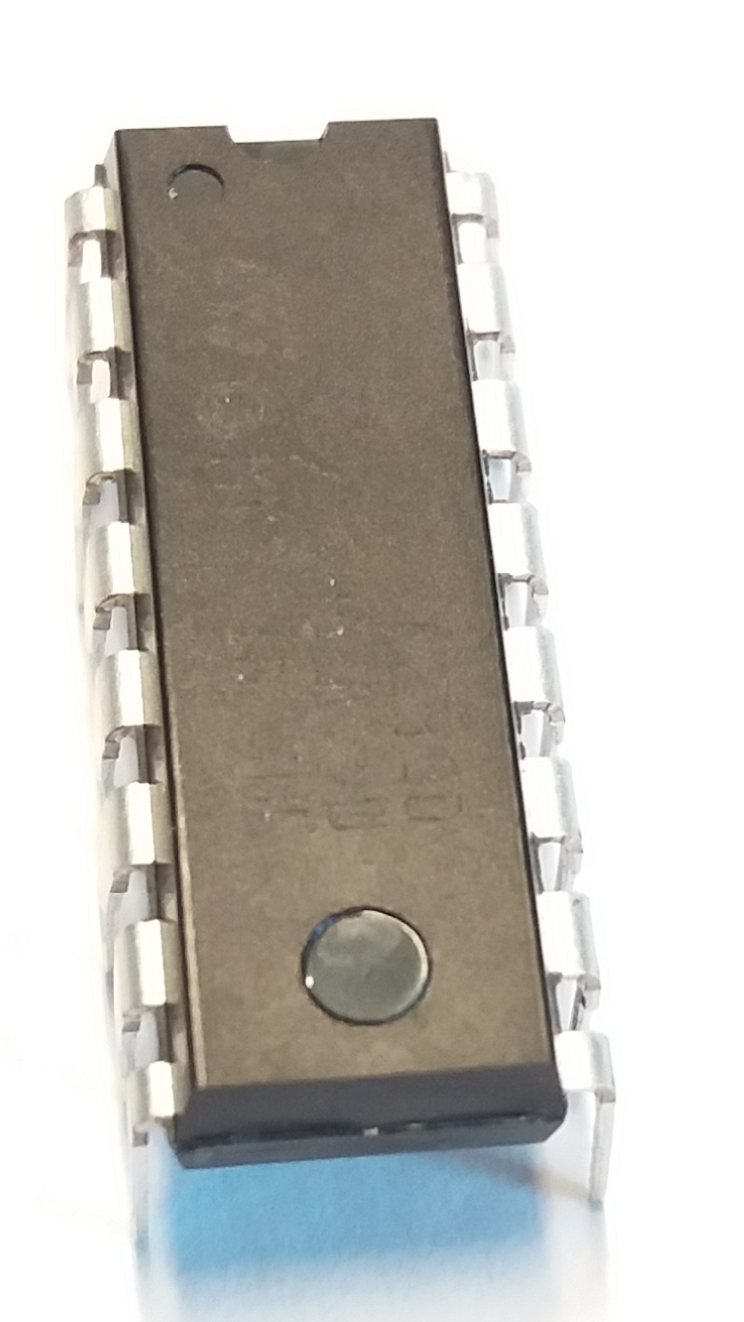
\includegraphics[width=0.8\textwidth]{./pics/l293d.jpg}
		\end{minipage}
		\hfill
		\begin{minipage}{0.48\textwidth}
			\centering
			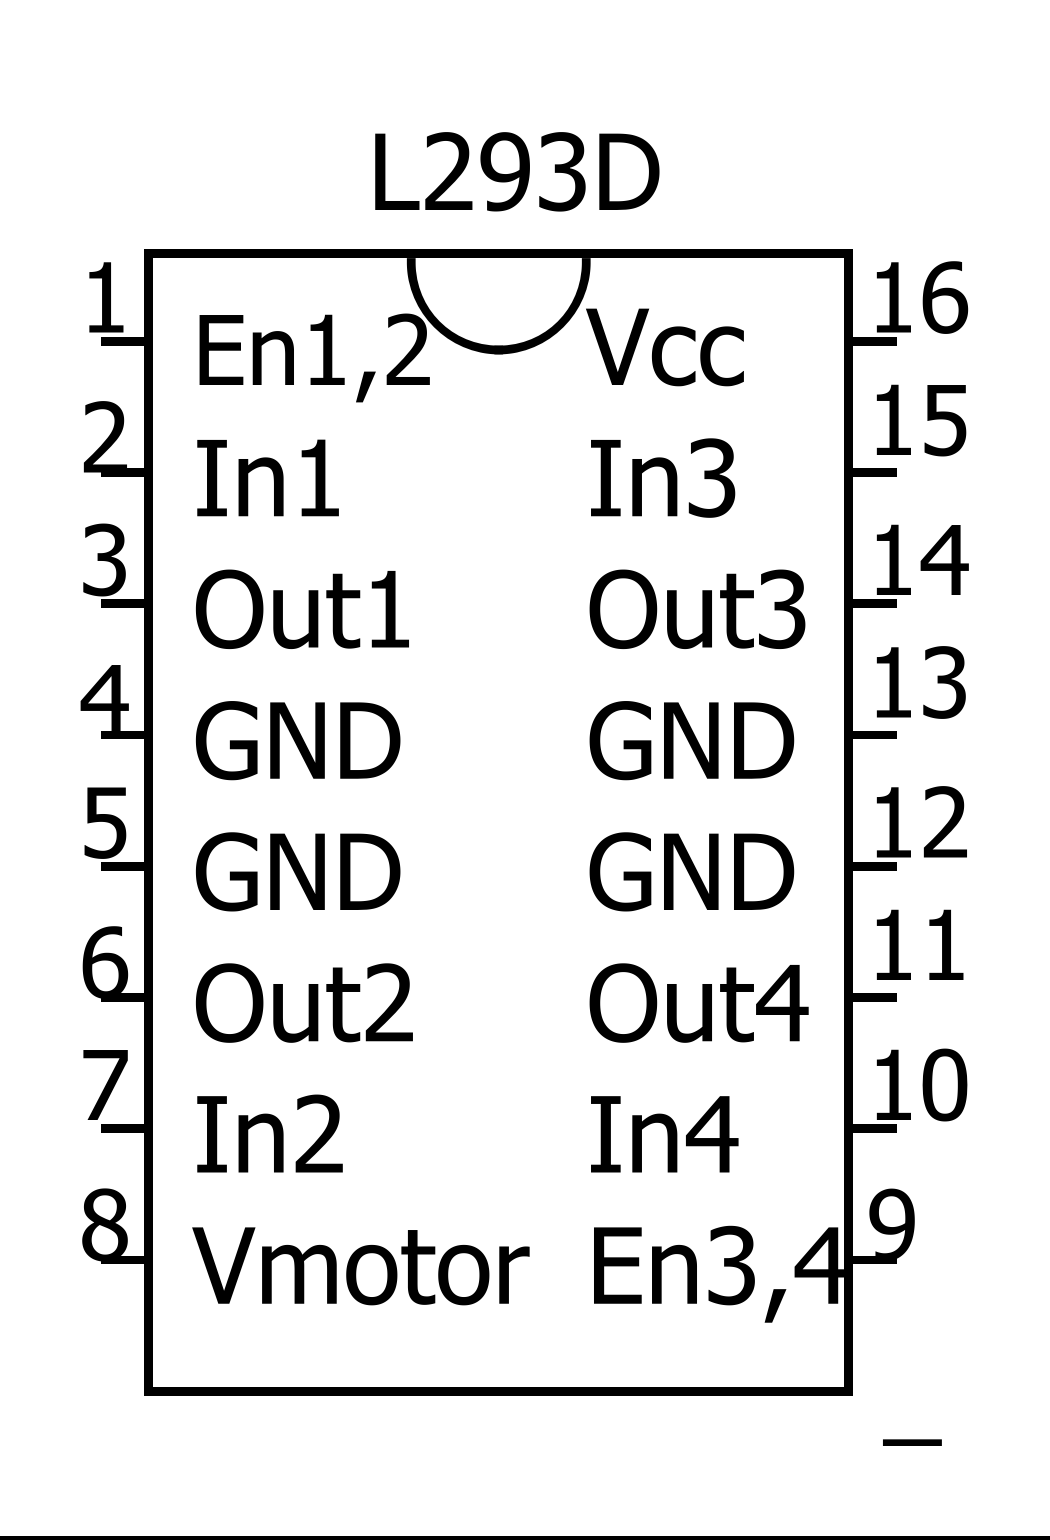
\includegraphics[width=\textwidth]{./Zeichnungen/motortreiber-l293d.png}
		\end{minipage}
	\end{minipage}

	\medskip		
	\emph{Achtung: Der L293D kann leicht mit anderen Bauteilen wie z.\,B. einem Shift-Register verwechselt werden, das dieselbe Bauart hat. Um sicher zu gehen, muss man die winzige Beschriftung des Bauteils lesen!}
\end{zsfg}

Im Folgenden wird die Belegung der Pins für die linke Seite beschrieben (vgl. Abbildung \ref{abb:l293d-an-arduino}). Die Belegung auf der rechten Seite verläuft analog.

Der Motor wird an Pin 3 und 6 (\texttt{Out1} und \texttt{Out2}) angeschlossen. Der jeweilige Zustand der \texttt{Out}-Pins kann über Pin 2 und 7 (\texttt{In1} und \texttt{In2}) geregelt werden. Wenn an \texttt{In1} der Zustand \texttt{HIGH} und an \texttt{In2} \texttt{LOW} anliegt, wird das auf \texttt{Out1} und \texttt{Out2} übertragen, sodass durch den Motor ein Strom fließen kann. Diese Übertragung wird jedoch durch Pin 1 (\texttt{En1,2} für \emph{enable pin 1, 2}) gesteuert. Wenn an \texttt{En1,2} \texttt{HIGH} anliegt, wird die Input-Konfiguration übertragen, bei \texttt{LOW} nicht. Durch ein PWM-Signal an \texttt{En1,2} kann die Leistung des Motors entsprechend gedrosselt werden.

Die vier \texttt{GND}-Anschlüsse dienen zur Stromversorgung und zur Wärmeableitung, falls hohe Ströme auftreten. An \texttt{Vmotor} wird der Pluspol der Versorgungsspannung für den Motor angeschlossen; an \texttt{Vcc} der Logik-Pegel von 5V für die Schaltung des IC.

\begin{figure}[H]
	\centering
	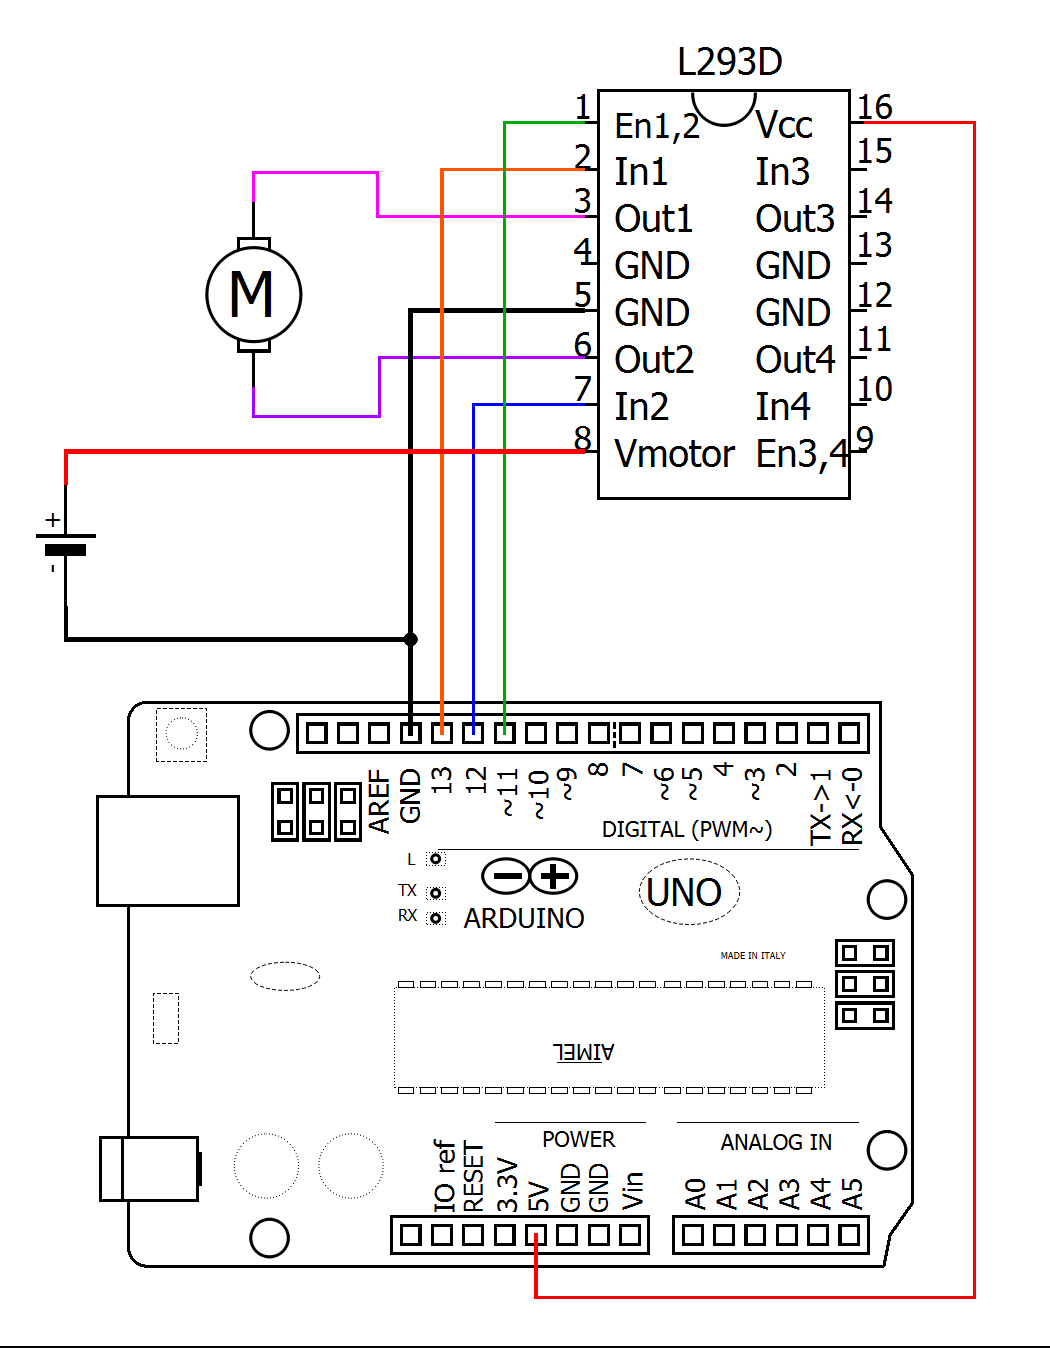
\includegraphics[width=0.5\textwidth]{./Zeichnungen/l293d-an-arduino.png}
	\caption{Steuerung eines Motors mit dem L293D.}
	\label{abb:l293d-an-arduino}
\end{figure}

% Pin-Belegung des IC

\begin{aufgabe} \emph{Betrieb des L293D}
	
	\medskip
	\begin{minipage}{0.53\textwidth}
		\begin{enumerate}[label=\alph*), itemsep=0mm, parsep=0mm]
			\item Baue die oben beschriebene Schaltung auf. Nutze dazu das \emph{Power Supply Module} (siehe S. \pageref{powersupplymodule}).
			\item Experimentiere mit verschiedenen Input-Konfigurationen und PWM-Werten für den \texttt{En1,2}-Pin. 
			
			\item Halte die Wirkung auf den Motor tabellarisch fest. Hier genügt es, wenn für den \texttt{En1,2}-Pin nur zwischen \emph{ein / 1} und \emph{aus / 0} unterschieden wird.
			
			\begin{tabular}{c|c|c|c}
				In1 & In 2 & En1,2 & Wirkung \\ \hline
				1 & 0 & 1 & \dots \\
			\end{tabular}
		\end{enumerate}
	\end{minipage}
	\hfill
	\begin{minipage}{0.45\textwidth}
		\begin{figure}[H]
			\centering
			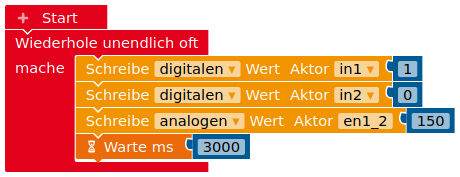
\includegraphics[width=0.9\textwidth]{./pics/prog-motorsteuerung-l293d.png}
		\end{figure}
	\end{minipage}
\end{aufgabe}
% Anschluss am Arduino und Aufbau der Schaltung sowie Test mit einfachem Programm
% Aufgabe: Alle Kombinationen durchprobieren und tabellarisch festhalten

\begin{recherche}{Wie stark darf der L293D belastet werden?}
	Bei Motoren ist immer genau darauf zu achten, welche Stromstärken und Spannungen die verwendeten Bauteile aushalten. Suche nach dem Datenblatt (\emph{data sheet}) des L293D und notiere die Maximalwerte zu Versorgungsspannung, Stromstärke und kurzfristige Spitzenstromstärke, die der IC aushält (\emph{absolute maximum ratings}). 
\end{recherche}
% Recherche: Absolute maximum ratings


\vfill
\begin{links}
	\item \href{https://www.instructables.com/id/Self-Driving-Car-Using-Arduinoautonomous-Guided-Ve/}{Autonomes Auto}
	
	Der Bastler hinter diesem Projekt hat einen Arduino-basierten Prototypen für ein autonomes Auto entworfen.
	
	\item \href{https://www.instructables.com/id/Arduino-Controlled-Game-Pong-Bot-Vs-Human/}{Pong-Bot}
	
	Ein kleines witziges Spiel hat dieser Bastler mit einem Arduino automatisiert.
	
	\item \href{https://www.instructables.com/id/Snack-Vending-Machine-Powered-by-Arduino/}{Snack-Automat}
	
	Ein Arduino-basierter Snack-Automat!
\end{links}